\pdfminorversion=6
% ============================================================
%  main.tex - Présentation ENSAE
%  Impact des transferts de migrants sur la pauvreté
%  multidimensionnelle des enfants au Sénégal
%  Compilable avec : pdflatex main.tex  (deux passes)
% ============================================================
\documentclass[10pt,aspectratio=169]{beamer}

% -- Thème principal ----------------------------------------
\usetheme{Antibes}
\useoutertheme{tree}

% -- Palette bronze / noir ----------------------------------
\definecolor{marron}{RGB}{112,84,44}
\definecolor{marronmed}{RGB}{139,100,60}
\definecolor{dore}{RGB}{184,134,11}
\definecolor{dorepale}{RGB}{245,230,200}
\colorlet{mybronze}{marron}

\setbeamercolor{structure}{fg=mybronze}
\setbeamercolor{palette primary}{bg=black, fg=white}
\setbeamercolor{palette secondary}{bg=mybronze, fg=white}
\setbeamercolor{palette tertiary}{bg=black, fg=white}
\setbeamercolor{palette quaternary}{bg=mybronze, fg=white}
\setbeamercolor{titlelike}{parent=palette secondary}
\setbeamercolor{headline}{bg=black, fg=white}
\setbeamercolor{frametitle}{bg=mybronze, fg=white}
\setbeamercolor{title}{fg=white}
\setbeamercolor{subtitle}{fg=dorepale}
\setbeamercolor{section in head/foot}{bg=black, fg=white}
\setbeamercolor{subsection in head/foot}{bg=mybronze, fg=white}
\setbeamercolor{block title}{bg=mybronze, fg=white}
\setbeamercolor{block body}{bg=dorepale, fg=black}
\setbeamercolor{block title alerted}{bg=marronmed, fg=white}
\setbeamercolor{block body alerted}{bg=dorepale!60, fg=black}
\setbeamercolor{alerted text}{fg=dore}
\setbeamercolor{item}{fg=mybronze}
\setbeamercolor{subitem}{fg=marronmed}


% -- Page de garde personnalisée avec TikZ ------------------
\setbeamercolor{author}{fg=black}
\setbeamercolor{institute}{fg=gray!70!black}

\makeatletter
\setbeamertemplate{title page}{%
  \begin{tikzpicture}[remember picture,overlay]
    \fill[mybronze!7] (current page.south west) rectangle (current page.north east);
    \fill[white] (current page.north west) rectangle ([yshift=-1.05cm]current page.north east);
    \fill[mybronze] ([yshift=-1.05cm]current page.north west) rectangle ([yshift=-1.17cm]current page.north east);
    \fill[white,rounded corners=18pt] ([xshift=1.05cm,yshift=-1.48cm]current page.north west)
      rectangle ([xshift=-1.05cm,yshift=0.70cm]current page.south east);
    \draw[mybronze!24,line width=0.9pt,rounded corners=18pt] ([xshift=1.05cm,yshift=-1.48cm]current page.north west)
      rectangle ([xshift=-1.05cm,yshift=0.70cm]current page.south east);
    \node[opacity=0.038] at ([yshift=-0.18cm]current page.center)
      {
\includegraphics[width=0.50\paperwidth]{prism-uploads/ENSAE.png}};
    \fill[black,opacity=0.10,rounded corners=12pt] ([xshift=1.0cm,yshift=-3.28cm]current page.north west)
      rectangle ([xshift=-1.0cm,yshift=-4.96cm]current page.north east);
    \fill[mybronze,rounded corners=12pt] ([xshift=1.02cm,yshift=-3.20cm]current page.north west)
      rectangle ([xshift=-1.02cm,yshift=-4.86cm]current page.north east);
    \draw[dore!85,line width=0.9pt,rounded corners=12pt] ([xshift=1.17cm,yshift=-3.25cm]current page.north west)
      rectangle ([xshift=-1.17cm,yshift=-4.81cm]current page.north east);
    \fill[dore!60,rounded corners=2pt] ([xshift=1.54cm,yshift=-4.82cm]current page.north west)
      rectangle ([xshift=-1.54cm,yshift=-4.91cm]current page.north east);
    \fill[white,opacity=0.10] ([xshift=1.0cm,yshift=-3.20cm]current page.north west)
      rectangle ([xshift=1.50cm,yshift=-4.86cm]current page.north west);
    \fill[white,opacity=0.08] ([xshift=-1.50cm,yshift=-3.20cm]current page.north east)
      rectangle ([xshift=-0.95cm,yshift=-4.86cm]current page.north east);
    \node[anchor=west,text=black,font=\scriptsize\bfseries] at ([xshift=0.55cm,yshift=-0.52cm]current page.north west) {Présentation du mémoire};
    \node[anchor=east,text=black,font=\scriptsize\bfseries] at ([xshift=-0.55cm,yshift=-0.52cm]current page.north east) {ENSAE Pierre Ndiaye};

  \end{tikzpicture}%

  \begin{center}
    \vspace{-0.1cm}
    
\includegraphics[width=0.13\paperwidth,height=2cm]{prism-uploads/ENSAE.png}\par
    \vspace{0.06cm}
    {\small\textcolor{gray!65!black}{École Nationale de la Statistique et de l'Analyse Économique}}\par
    {\small\textcolor{gray!65!black}{Pierre Ndiaye}}\par

    \vspace{0.44cm}
    \begin{minipage}{0.84\paperwidth}
      \centering
      {\usebeamerfont{title}\bfseries\color{white}\inserttitle\par}%
    \end{minipage}\par

    \vspace{0.55cm}
    \hspace{-7cm}{\scriptsize\textcolor{gray!70!black}{Présenté par :}}\par
    \vspace{0.03cm}
    {\small\textcolor{mybronze}{\textbf{Sié Rachid TRAORÉ}}}\par
    \vspace{0.04cm}
    {\small\textcolor{gray!70!black}{Élève Ingénieur Statisticien Économiste en fin de formation}}\par

    \vspace{0.16cm}
    \hspace{-5cm}{\scriptsize\textcolor{gray!70!black}{Sous la direction de}}\par
    \vspace{0.03cm}
    {\small\textcolor{mybronze}{\textbf{Mamadou Abdoulaye DIALLO}}}\par
    \vspace{0.03cm}
    {\small\textcolor{gray!70!black}{Chercheur postdoctoral en économie appliquée, ISE}}\par

    \vfill
    {\small\textcolor{mybronze}{\textbf{\insertdate}}}\par
    \vspace{0.12cm}
  \end{center}%
}
\makeatother

% -- Pied de page --------------------------------------------
\setbeamertemplate{footline}{%
  \leavevmode%
  \begin{beamercolorbox}[wd=.33\paperwidth,ht=2.25ex,dp=1ex,left]{palette secondary}%
    \hspace{0.3cm}\tiny Diapositive~\insertframenumber/\inserttotalframenumber%
  \end{beamercolorbox}%
  \begin{beamercolorbox}[wd=.34\paperwidth,ht=2.25ex,dp=1ex,center]{palette secondary}%
    \tiny\insertshortauthor%
  \end{beamercolorbox}%
  \begin{beamercolorbox}[wd=.33\paperwidth,ht=2.25ex,dp=1ex,right]{palette secondary}%
    \tiny ENSAE Pierre Ndiaye\hspace{0.3cm}
  \end{beamercolorbox}%
}

% -- Symboles de navigation supprimés -----------------------
\setbeamertemplate{navigation symbols}{}

% -- Légendes numérotées ------------------------------------
\setbeamertemplate{caption}[numbered]

% -- Blocs avec coins arrondis ------------------------------
\setbeamertemplate{blocks}[rounded][shadow=false]

% -- Puces --------------------------------------------------
\setbeamertemplate{itemize item}{\color{marron}$\blacktriangleright$}
\setbeamertemplate{itemize subitem}{\color{dore}$\triangleright$}

% -- Packages -----------------------------------------------
\usepackage[T1]{fontenc}
\usepackage[utf8]{inputenc}
\usepackage[french]{babel}
\usepackage{amsmath,amssymb,amsfonts}
\usepackage{booktabs}
\usepackage{graphicx}
\usepackage{array}
\usepackage{colortbl}
\usepackage{multirow}
\usepackage{ragged2e}
\usepackage{tikz}
\usetikzlibrary{positioning,arrows.meta,shapes}

% -- Justification des textes --------------------------------
\AtBeginEnvironment{frame}{\justifying}
\addtobeamertemplate{block begin}{}{\justifying}
\addtobeamertemplate{block alerted begin}{}{\justifying}
\addtobeamertemplate{block example begin}{}{\justifying}

% -- Métadonnées --------------------------------------------
\title[Impact des transferts de migrants sur la pauvreté des enfants]{%
  Impact des transferts de migrants sur la pauvreté multidimensionnelle des enfants au Sénégal}
\author[Sié\,Rachid TRAORÉ]{Sié Rachid TRAORÉ}
\institute[ENSAE]{%
  École Nationale de la Statistique et de l'Analyse Économique\\
  Pierre Ndiaye (ENSAE)}
\date{Juillet 2026}

% ============================================================
\begin{document}
% ============================================================

% -- Page de garde (sans en-tête) ----------------------------
\begin{frame}[plain,noframenumbering]
  \titlepage
\end{frame}

% -- Plan ----------------------------------------------------
\begin{frame}{Plan de la présentation}
  \tableofcontents[hideallsubsections]
\end{frame}

% ============================================================
\section[Introduction]{Introduction}
% ============================================================

\subsection{Contexte et motivation}

\begin{frame}{Contexte général}
  \begin{block}{Place des transferts de migrants dans l'économie sénégalaise}
    \begin{itemize}
      \item Les transferts de fonds représentent environ \textbf{10-12\,\%} du PIB sénégalais.
      \item Première source de devises, devançant l'aide publique au développement et les IDE.
      \item Plus de \textbf{3 millions} de Sénégalais vivent à l'étranger (diaspora).
      \pause
    \end{itemize}
  \end{block}
  \begin{alertblock}{Pauvreté infantile : un défi persistant}
    \begin{itemize}
      \item Près de \textbf{64\,\%} des enfants souffrent de privations multiples (N-MODA, EHCVM I, effectifs bruts).
      \item Privations cumulées : éducation, santé, eau, assainissement, logement, nutrition, protection.
      \item La pauvreté monétaire ne suffit pas à capturer toutes ces dimensions.
    \end{itemize}
  \end{alertblock}
\end{frame}

\subsection{Problématique et objectifs}

\begin{frame}{Problématique}
  \begin{block}{Question de recherche}
    \justifying
    \large
    \textit{Dans quelle mesure les transferts de migrants réduisent-ils
    la \textbf{pauvreté multidimensionnelle} des enfants au Sénégal ?}
  \end{block}
  \medskip
  \begin{block}{Enjeu méthodologique}
    Les ménages bénéficiaires de transferts \textbf{ne sont pas un échantillon aléatoire} :
    biais de sélection observable et inobservable.
  \end{block}
  \begin{alertblock}{Réponse méthodologique}
    Combinaison \textbf{PSM + Double différence} sur les données \textbf{EHCVM I \& II} (2018-2022).
  \end{alertblock}
\end{frame}

\begin{frame}{Objectifs et hypothèses}
  \begin{block}{Objectif général}
    Évaluer l'impact causal des transferts de migrants sur la pauvreté
    multidimensionnelle des enfants au Sénégal.
  \end{block}
  \pause
  \begin{block}{Objectifs spécifiques}
    \begin{itemize}
      \item Mesurer la pauvreté multidimensionnelle des enfants selon l'approche N-MODA (EHCVM I \& II).
      \item Analyser son évolution entre 2018-2019 et 2021-2022.
      \item Estimer l'effet causal des transferts par PSM-Double différence.
    \end{itemize}
  \end{block}
  \pause
  \begin{block}{Hypothèses de recherche}
    \begin{enumerate}
      \item[H1] Les transferts réduisent significativement la pauvreté multidimensionnelle des enfants.
      \item[H2] L'effet est \textbf{hétérogène} selon les dimensions et le milieu de résidence.
      \item[H3] Le PSM-DD contrôle efficacement les biais de sélection observés et inobservés.
    \end{enumerate}
  \end{block}
\end{frame}

% ============================================================
\section[Revue]{Revue de la littérature}
% ============================================================

\subsection{Transferts de migrants et bien-être}

\begin{frame}{Transferts de migrants : canaux de transmission}
  \begin{block}{Théories sur les transferts}
    \begin{itemize}
      \item \textbf{Altruisme} (Lucas \& Stark, 1985) : les migrants soutiennent leur famille par solidarité.
      \item \textbf{Contrat familial implicite} : les transferts compensent l'investissement consenti dans la migration.
      \item \textbf{Diversification des risques} : le ménage envoie un membre migrer pour sécuriser les revenus.
    \end{itemize}
  \end{block}
  \pause
  \begin{block}{Effets empiriques documentés}
    \begin{itemize}
      \item Réduction de la pauvreté monétaire (Adams \& Page, 2005 ; Acosta et al., 2008).
      \item Amélioration de la scolarisation et de la santé des enfants (Yang, 2008).
      \item Effets plus marqués en milieu rural et pour les ménages les plus pauvres.
    \end{itemize}
  \end{block}
\end{frame}

\subsection{Pauvreté multidimensionnelle des enfants}

\begin{frame}[shrink=8]{Approche multidimensionnelle de la pauvreté infantile}
  \begin{block}{Limites de l'approche monétaire}
    \begin{itemize}
      \item Le revenu/la consommation ne capturent pas toutes les privations des enfants.
      \item Les enfants ont des besoins spécifiques : nutrition, éducation, soins de santé.
    \end{itemize}
  \end{block}
  \begin{alertblock}{L'approche Alkire-Foster (2011)}
    \begin{itemize}
      \item Identification des privations dans plusieurs dimensions simultanément.
      \item Double seuil : intra-dimensionnel (seuil de privation) et inter-dimensionnel (seuil de pauvreté $k$).
      \item Mesure $M_0 = H \times A$ : incidence $\times$ intensité.
    \end{itemize}
  \end{alertblock}
  \begin{block}{Lacune dans la littérature}
    Peu d'études combinent PSM et double différence pour identifier l'effet causal
    des transferts sur la pauvreté \textbf{multidimensionnelle} des enfants au Sénégal.
  \end{block}
\end{frame}

% ============================================================
\section[Méthodologie]{Cadre méthodologique}
% ============================================================

\subsection{Mesure de la pauvreté multidimensionnelle}

\begin{frame}[shrink=8]{N-MODA : 7 dimensions, 3 groupes d'âge}
  \begin{block}{Méthodologie N-MODA (ANSD/UNICEF)}
    \centering\smallskip
    \begin{tabular}{llccc}
      \toprule
      Dimension    & Indicateurs principaux           & 0-4 & 5-14 & 15-17 \\
      \midrule
      Assainissement & Toilettes non améliorées / partagées & \checkmark & \checkmark & \checkmark \\
      Eau          & Source non améliorée / accès $>30$ min & \checkmark & \checkmark & \checkmark \\
      Logement     & Ordures non saines / surpeuplement   & \checkmark & \checkmark & \checkmark \\
      Nutrition    & Diversité des repas / sécurité alim.  & \checkmark & \checkmark & \checkmark \\
      Santé        & Combustible solide / accès aux soins  & \checkmark & \checkmark & \checkmark \\
      Protection   & Acte de naissance / travail enfants   & \checkmark & \checkmark & \checkmark \\
      Éducation    & Non-scolarisation / illettrisme / NEET & - & \checkmark & \checkmark \\
      \bottomrule
    \end{tabular}
  \end{block}
  \begin{alertblock}{Double seuil N-MODA}
    Union intra-dimension (privé si privé dans au moins un indicateur) ;
    seuil inter-dimensionnel $k = 4$ (pauvre si privé dans $\geq 4$ dimensions sur 7).
  \end{alertblock}
\end{frame}

\begin{frame}[shrink=8]{Le traitement : les transferts de migrants en pratique}
  \begin{block}{Motifs déclarés des transferts étrangers (EHCVM I / II, \% des transferts)}
    \centering\smallskip
    \begin{tabular}{lcc}
      \toprule
      Motif principal & 2018 & 2021 \\
      \midrule
      Soutien courant            & 66,7\,\% & 68,5\,\% \\
      Fête, évènements           & 11,3\,\% & 9,3\,\% \\
      Santé, maladie             & 4,6\,\%  & 6,5\,\% \\
      Scolarité, éducation       & 3,5\,\%  & 3,7\,\% \\
      Autres motifs              & 13,9\,\% & 12,0\,\% \\
      \bottomrule
    \end{tabular}
  \end{block}
  \begin{alertblock}{Montants annuels reçus par ménage bénéficiaire}
    Médiane $\approx$ 300\,000 FCFA/an ; moyenne $\approx$ 900\,000 FCFA/an
    (forte dispersion) : une ressource loin d'être marginale.
  \end{alertblock}
  \begin{block}{Implication méthodologique}
    Deux tiers des transferts relèvent du soutien courant, non affecté :
    l'argent étant fongible, on mesure l'effet sur les \textbf{privations
    effectives} des enfants plutôt que sur l'affectation déclarée des fonds.
  \end{block}
\end{frame}

\subsection{Stratégie d'identification}

\begin{frame}[shrink=25]{PSM + Double différence : principe}

  \begin{alertblock}{Traitement : design entrants (DD canonique)}
    Traités = ménages \textbf{entrants} (aucun transfert étranger en 2018,
    transfert reçu en 2021) ; témoins = jamais bénéficiaires. Les ménages
    déjà bénéficiaires en 2018 sont exclus : la période de base précède le
    début du traitement.
  \end{alertblock}

  \begin{block}{Problème du biais de sélection}
    L'effet moyen du traitement sur les traités (ATT) :
    \begin{equation*}
      \tau_{ATT} = \mathbb{E}[Y_i(1) - Y_i(0) \mid D_i = 1]
    \end{equation*}
    $Y_i(0)$ (contrefactuel) est inobservable $\Rightarrow$ nécessité d'un estimateur adapté.
  \end{block}

  \begin{block}{Étape 1 - Appariement par score de propension (PSM)}
    Estimation du score de propension par probit :
    \begin{equation*}
      p(X_i) = P(D_i = 1 \mid X_i) = \Phi(X_i'\beta)
    \end{equation*}
    Appariement par $k$-plus proches voisins ($k=4$) et vérification du support commun.
  \end{block}

  \begin{alertblock}{Étape 2 - Double différence (DD) après appariement}
    \begin{equation*}
      \hat{\tau}_{PSM\text{-}DD}
      = \frac{1}{n_T}\sum_{i\in\mathcal{T}}
        \Bigl[\underbrace{Y_{i,t_2}-Y_{i,t_1}}_{\Delta Y_i}
        - \sum_{j\in\mathcal{C}} w_{ij}\,\Delta Y_j\Bigr]
    \end{equation*}
    Contrôle simultané des biais observables (PSM) et des effets fixes inobservés (DD).
  \end{alertblock}
\end{frame}

\subsection{Données EHCVM}

\begin{frame}{Données : EHCVM I et II}
  \begin{block}{Source et période}
    \begin{itemize}
      \item \textbf{EHCVM I (2018-2019)} : première vague harmonisée UEMOA au Sénégal.
      \item \textbf{EHCVM II (2021-2022)} : deuxième vague permettant de constituer un panel.
      \item \textbf{Panel vrai} : 6\,127 ménages suivis entre les deux vagues.
      \item \textbf{Traitement (entrants)} : 816 ménages devenus bénéficiaires
            en 2021, comparés à 3\,981 ménages jamais bénéficiaires.
    \end{itemize}
  \end{block}
  \begin{block}{Population cible}
    Enfants de \textbf{0 à 17 ans} résidant dans les ménages appariés entre les deux vagues.
  \end{block}
  \begin{alertblock}{Covariables du modèle de propension}
    Âge, sexe et niveau d'éducation du chef de ménage ; taille du ménage ;
    milieu de résidence (urbain/rural) ; région ; possession d'actifs.
  \end{alertblock}
\end{frame}

% ============================================================
\section[Résultats]{Résultats empiriques}
% ============================================================

\subsection{État de la pauvreté multidimensionnelle}

\begin{frame}{Pauvreté multidimensionnelle des enfants : état des lieux}
  \begin{columns}
    \begin{column}{0.48\textwidth}
      \begin{block}{Résultats N-MODA ($k=4$)}
        \centering\smallskip
        \begin{tabular}{lccc}
          \toprule
          Vague & $H$ & $A$ & $M_0$ \\
          \midrule
          2018-2019 & 63,6\,\% & 70,2\,\% & 0,447 \\
          2021-2022 & 55,3\,\% & 68,6\,\% & 0,380 \\
          \midrule
          $\Delta$ & $-8{,}3$ pp & $-1{,}6$ pp & $-0{,}067$ \\
          \bottomrule
        \end{tabular}
      \end{block}
      \begin{block}{Lecture}
        La pauvreté recule nettement en incidence, mais l'intensité reste
        quasi stable : les enfants pauvres cumulent toujours près de 5
        privations sur 7.
      \end{block}
    \end{column}
    \begin{column}{0.50\textwidth}
      \centering
      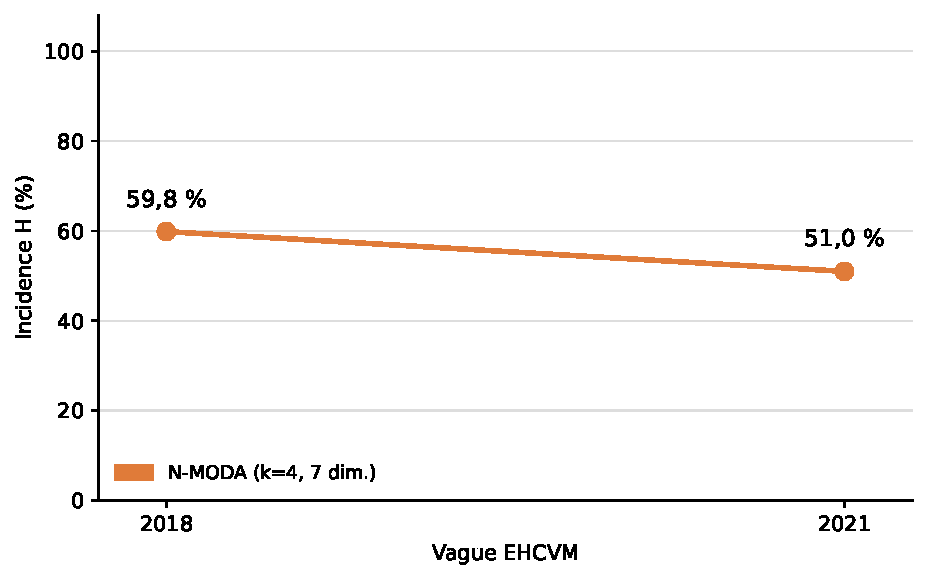
\includegraphics[width=\linewidth]{figures/fig_evolution_ipm.pdf}
    \end{column}
  \end{columns}
\end{frame}

\begin{frame}{Privations par dimension (N-MODA)}
  \begin{columns}
    \begin{column}{0.50\textwidth}
      \centering
      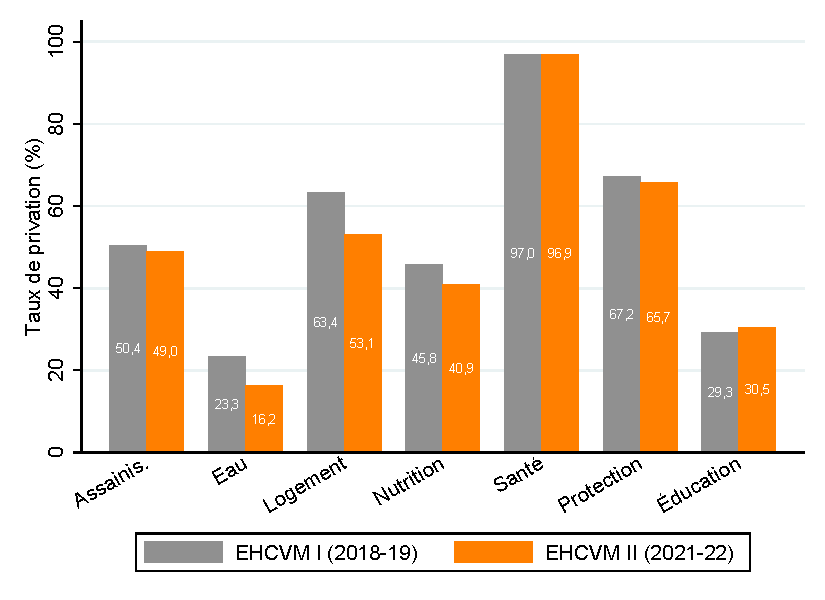
\includegraphics[width=\linewidth]{figures/fig_privations_dim.pdf}
    \end{column}
    \begin{column}{0.48\textwidth}
      \centering
      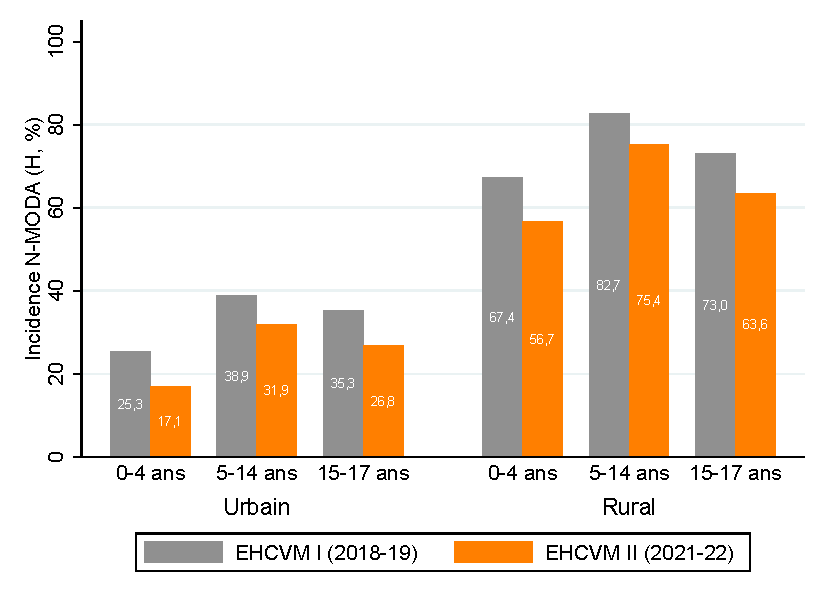
\includegraphics[width=\linewidth]{figures/fig_pauvrete_milieu_age.pdf}
    \end{column}
  \end{columns}
  \begin{alertblock}{Amélioration entre 2018 et 2022}
    Baisse de 8,3 pp de l'incidence N-MODA ;
    plus d'un enfant sur deux reste privé dans au moins 4 dimensions.
  \end{alertblock}
\end{frame}

\subsection{Qualité de l'appariement}

\begin{frame}{Qualité de l'appariement PSM}
  \begin{columns}
    \begin{column}{0.52\textwidth}
      \centering
      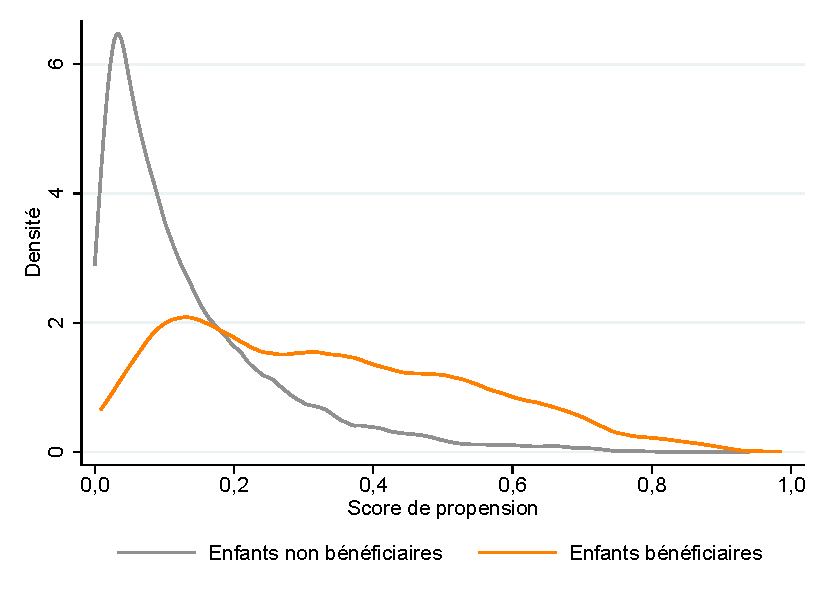
\includegraphics[width=\linewidth]{figures/overlap.pdf}
    \end{column}
    \begin{column}{0.46\textwidth}
      \begin{block}{Équilibre après appariement ($k$-NN, $k=4$)}
        \begin{itemize}
          \item Probit peu prédictif (pseudo-$R^2 = 0{,}042$) : sélection
                initiale modérée, cohérente avec un traitement débutant
                après la période de base.
          \item Biais standardisé moyen : 7,7\,\% avant, \textbf{1,4\,\%}
                après appariement.
          \item 784 ménages entrants, tous sur support commun, appariés à
                1\,863 témoins distincts.
        \end{itemize}
      \end{block}
    \end{column}
  \end{columns}
\end{frame}

\subsection{Impact des transferts}

\begin{frame}[shrink=15]{Impact des transferts sur la pauvreté multidimensionnelle}
  \begin{table}
    \centering
    \caption{Effet moyen sur les traités (ATT), pauvreté N-MODA}
    \renewcommand{\arraystretch}{1.3}
    \begin{tabular}{lccc}
      \toprule
      Spécification & ATT & Éc.-t. & $p$-valeur \\
      \midrule
      DD brute (sans appariement)      & $0{,}001$ & (0,022) & 0,976 \\
      \textbf{PSM-DD, k-NN ($k=4$)}   & $\mathbf{0{,}010}$ & (0,026) & \textbf{0,707} \\
      PSM-DD, noyau Epanechnikov       & $0{,}005$ & (0,023) & 0,822 \\
      PSM-DD, caliper                  & $0{,}010$ & (0,030) & 0,744 \\
      \bottomrule
    \end{tabular}
  \end{table}
  \begin{alertblock}{Résultat central : aucun effet détectable à court terme}
    Sur 2018-2021, la pauvreté multidimensionnelle des enfants des ménages
    devenus bénéficiaires recule \emph{au même rythme} que celle des témoins
    appariés. Conclusion robuste aux quatre spécifications.
  \end{alertblock}
  \begin{block}{Lecture}
    Trois mécanismes : délai de matérialisation (privations structurelles vs
    exposition $<$ 3 ans), compensation entre canaux (apport monétaire vs
    coûts du départ du migrant), contraintes d'offre de services de base.
  \end{block}
\end{frame}

\begin{frame}{Effets par dimension de la pauvreté}
  \begin{columns}
    \begin{column}{0.55\textwidth}
      \centering
      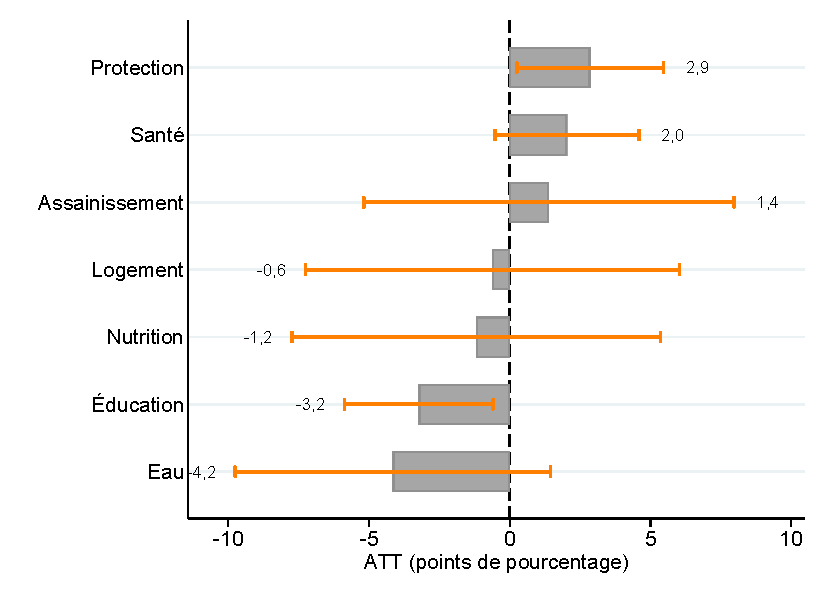
\includegraphics[width=\linewidth]{figures/fig_effets_dim.pdf}
    \end{column}
    \begin{column}{0.43\textwidth}
      \begin{alertblock}{Deux canaux opposés qui se compensent}
        \begin{itemize}
          \item \textbf{Éducation} : $-3{,}2$ pp ($p=0{,}017$),
                seule dimension en amélioration significative.
          \item \textbf{Protection de l'enfant} : $+2{,}9$ pp
                ($p=0{,}032$), dégradation liée à la séparation
                parentale qui accompagne le départ du migrant.
          \item Les cinq autres dimensions : aucun effet significatif.
        \end{itemize}
      \end{alertblock}
    \end{column}
  \end{columns}
  \begin{block}{Lecture : preuve directe du mécanisme de compensation}
    Le résultat nul agrégé masque deux effets sectoriels de signes opposés
    et d'ampleurs comparables : le bénéfice éducatif de l'apport monétaire
    (cohérent avec les motifs déclarés) est neutralisé par le coût de
    l'absence parentale. Aucune différence par milieu, sexe ou âge.
  \end{block}
\end{frame}

% ============================================================
\section[Robustesse]{Robustesse et discussion}
% ============================================================

\subsection{Tests de robustesse}

\begin{frame}{Tests de robustesse}
  \begin{block}{Sensibilité des résultats}
    \begin{itemize}
      \item Méthodes d'appariement (k-NN, noyau, caliper) et DD brute :
            conclusion nulle identique dans les quatre cas.
      \item Panel d'enfants (mêmes enfants suivis entre les vagues) :
            ATT $= 0{,}015$ ($p=0{,}576$), pas d'artefact de composition par âge.
      \item Test placebo (200 assignations aléatoires) : l'ATT réel se situe au
            63\textsuperscript{e} centile de la distribution placebo,
            indiscernable du hasard.
    \end{itemize}
  \end{block}
  \begin{alertblock}{Définition alternative : les bénéficiaires durables}
    Chez les ménages bénéficiaires aux deux vagues (traitement antérieur à la
    base), la dynamique relative est défavorable et significative
    ($0{,}089$, $p=0{,}018$) : les effets des transferts, dans un sens comme
    dans l'autre, se matérialisent au-delà de l'horizon de trois ans.
  \end{alertblock}
\end{frame}

\begin{frame}{Validation des hypothèses - Synthèse}
  \begin{table}
    \centering
    \caption{Bilan des hypothèses de recherche}
    \renewcommand{\arraystretch}{2}
    \begin{tabular}{c p{3.5cm} p{5.5cm} c}
      \toprule
      Hyp. & Énoncé & Résultat & Décision \\
      \midrule
      H1 & Réduction de la pauvreté & ATT N-MODA $= 0{,}010$ ($p=0{,}707$) : pas d'effet à court terme & Non rejet de $H_0$ \\[4pt]
      H2 & Hétérogénéité des effets  & Éducation favorable vs protection dégradée ; rien par milieu, sexe ou âge & Partiellement \\[4pt]
      H3 & PSM-DD contrôle les biais & Support commun total ; biais moyen 1,4\,\% après appariement & Confirmée \\
      \bottomrule
    \end{tabular}
  \end{table}
\end{frame}

% ============================================================
\section[Conclusion]{Conclusion et recommandations}
% ============================================================

\subsection{Conclusion générale}

\begin{frame}{Conclusion générale}
  \begin{block}{Principaux apports}
    \begin{enumerate}
      \item Mesure de la pauvreté multidimensionnelle des enfants sur deux
            vagues EHCVM selon l'approche N-MODA (7 dimensions, $k=4$).
      \pause
      \item L'incidence N-MODA recule de 63,6\,\% (2018) à 55,3\,\% (2021) :
            amélioration réelle mais la pauvreté reste massive.
      \pause
      \item Devenir bénéficiaire de transferts ne modifie pas, à trois ans,
            la trajectoire de privations des enfants (ATT $0{,}010$,
            $p=0{,}707$, robuste aux quatre spécifications).
      \pause
      \item L'impact est différencié : l'éducation s'améliore
            ($-3{,}2$ pp) tandis que la protection se dégrade
            ($+2{,}9$ pp) - deux canaux opposés qui se compensent.
    \end{enumerate}
  \end{block}
\end{frame}

\subsection{Recommandations}

\begin{frame}{Recommandations de politique économique}
  \begin{block}{Faciliter et orienter les transferts}
    \begin{itemize}
      \item Réduire les coûts de transaction des envois de fonds formels.
      \item Encourager le fléchage des transferts vers l'éducation et la santé des enfants.
      \item Développer des produits d'épargne liés aux transferts pour les ménages ruraux.
    \end{itemize}
  \end{block}
  \pause
  \begin{block}{Renforcer les politiques sociales complémentaires}
    \begin{itemize}
      \item Accompagner les ménages nouvellement bénéficiaires dans la durée
            (inclusion financière, appui à l'investissement dans l'habitat).
      \item Améliorer l'offre de services publics (écoles, centres de santé) dans les zones d'émigration.
      \item Renforcer les systèmes de collecte de données sur les migrations et les transferts.
    \end{itemize}
  \end{block}
\end{frame}

\subsection{Limites et perspectives}

\begin{frame}[shrink=8]{Limites et perspectives de recherche}
  \begin{alertblock}{Limites de l'étude}
    \begin{itemize}
      \item Panel non cylindré : attrition sélective (ménages urbains et aisés).
      \item L'ATT capte l'effet conjoint du départ du migrant et des transferts ;
            durée d'exposition variable au sein des entrants (effet de court terme).
      \item Dimension nutrition limitée à la sécurité alimentaire (module FIES).
      \item Effets de spillover possibles entre ménages bénéficiaires et non-bénéficiaires.
    \end{itemize}
  \end{alertblock}
  \pause
  \begin{block}{Perspectives}
    \begin{itemize}
      \item Analyser les mécanismes de transmission (dépenses en éducation, santé, logement).
      \item Étendre l'analyse aux autres pays de l'UEMOA couverts par l'EHCVM.
      \item Intégrer la dimension genre de l'enfant et du chef de ménage.
    \end{itemize}
  \end{block}
\end{frame}

% -- Diapositive de clôture ----------------------------------
\begingroup
\setbeamertemplate{headline}{}
\setbeamertemplate{footline}{}
\begin{frame}[noframenumbering]
  \begin{center}
    \vspace{1.5cm}
    {\Huge\textcolor{marron}{\textbf{Merci de votre attention}}}\\[1cm]
    \begin{tikzpicture}
      \draw[marron,line width=2pt] (0,0) -- (8,0);
    \end{tikzpicture}\\[0.8cm]
    {\large\textit{Questions et échanges}}\\[1cm]
    \small
    \textbf{Sié Rachid TRAORÉ}\\[0.3cm]
    \textit{Sous la direction de Mamadou Abdoulaye DIALLO}\\[0.2cm]
    ENSAE Pierre Ndiaye - Juillet 2026
  \end{center}
\end{frame}
\endgroup

\end{document}
